% \begin{savequote}[8cm]
% Alles Gescheite ist schon gedacht worden.\\
% Man muss nur versuchen, es noch einmal zu denken.

% All intelligent thoughts have already been thought;\\
% what is necessary is only to try to think them again.
%   \qauthor{--- Johann Wolfgang von Goethe \cite{von_goethe_wilhelm_1829}}
% \end{savequote}

\chapter{\label{ch:2-draft}Active Phase Separation of Dense Mixtures}

\minitoc

\section{Introduction}

Aggregation and compartmentalisation within the cellular environment has been observed in a variety of contexts\cite{weber_drops_2021}. Droplet-like compartments can form reactors for certain cellular processes\cite{nott_phase_2015} or buffer noise in the cellular environment\cite{klosin_phase_2020} and aggregation of the $\alpha$-synuclein protein has strong links to the development of Parkinson's Disease\cite{tong_loss_2010}. Understanding the physical processes surrounding this phase separation and aggregation is nessecary to develop techniques to prevent or encourage this formation and may also identify further downstream consequences and effects.

A variety of both equilibrium and non-equilibrium mechanisms have been studied that can cause phase separation\cite{li_non-equilibrium_2020,weber_drops_2021}. Recently, the role chemical activity between the constituent components of a system have been explored and a rich phenomena beyond simple phase separation or aggregation can be observed \cite{agudo-canalejo_active_2019}. A potential limitation of these models may be their relevance to the exact values of system parameters which may not be found in the natural world. Conversely, enzymatic activity is ubiquitous and arguably necessary in living systems and an interesting question is whether this abundant activity can be a mechanism to cause such phase separation and aggregation.

\section{Equilibrium Phase Separation}

\subsection{Thermodynamics of Fluid Mixtures}

A good example to explore the theory of phase separating mixtures is to study a fluid made up of two components, say, component $A$ and component $B$. To make this mixture, we mix a $N_A$ molecules of component $A$ and $N_B$ molecules of component $B$ to give a mixture of total volume $V = v_A N_A + v_B N_B$, where $v_i$ is the specific volume of the component, the \textit{size} of each molecule. The volume fraction of a component, $\phi_i$, is defined to be $\phi_i = v_i N_i/v$ and for the two component mixture $\phi_A+\phi_B = 1$. To simplify the notation, let $\phi_A=\phi$ and $\phi_B=1-\phi$, and the volume fraction $\phi$ now describes the proportion of the fluid volume that is component $A$. For an incompressible fluid, the total volume is constant and the relevant free energy is the Helmholtz free energy, $F(N_A, N_B, T)$ where $T$ is the temperature of the fluid. The Helmholtz Free energy is an extensive quantity and so the $F(N_A, N_B, T) = V f(\phi, T)$ where $f(\phi, T)$ is the free energy density and this free energy density determines the phase behaviour of the mixture. The mixture will phase separate into two regions with different $\phi$s if this lowers the overall free energy. Labelling the two phases $\mathrm{I}$ and $\mathrm{II}$ the reduced free energy condition is $Vf(\phi, T) = V_{\mathrm{I}} f(\phi_{\mathrm{I}}, T)+ V_{\mathrm{II}} f(\phi_{\mathrm{II}}, T)$ with the total volume being conserved $V = V_{\mathrm{I}}+V_{\mathrm{II}}$. This is equivalent to the free energy density being upper convex, $\frac{\partial^2 f}{\partial \phi^2}$, for some value for $\phi$.

In addition to lowering the free energy of the system, any phase separating regions of a mixture must also be in mechanical and chemical equilibrium, otherwise they would exchange components or volume to reach two equilibrated phases. Chemical equilibrium is achieved when the chemical potential, $\mu$ of each component in each phase is constant and so moving a particle across the phase boundary will not change the free energy, $\mu_i^{\mathrm{I}}=\mu_i^{\mathrm{II}}$. The chemical potential for component $i$ is given by
\begin{equation}
    \mu_i = \left(\frac{\partial F}{\partial N_i}\right)_{V, T} = \left(\frac{\partial f}{\partial \phi_i}\right)_{T}.
    \label{eq:mu_def}
\end{equation}
\todo{Also need to get the volume dependency in here somehow.}
The mechanical equilibrium is achieved when the osmotic pressure, $\Pi$ between the two phases is equal, $\Pi^{\mathrm{I}}=\Pi^{\mathrm{II}}$, where the osmotic pressure is given by \todo{difference between osmotic and mechanical pressure}
\begin{equation}
    \Pi(\phi) = -\left(\frac{\partial F}{\partial V}\right)_{T, N_A} = -f + \phi \left(\frac{\partial f}{\partial \phi}\right)_{T}.
    \label{eq:Pi_def}
\end{equation}
These conditions have a convenient graphical interpretation. The equation for a tangent to the curve $f(\phi)$ at $\phi=\Tilde{\phi}$ can be written as $y=mx+c$. Equation (\ref{eq:mu_def}) and (\ref{eq:Pi_def}) give $y=\mu_A(\Tilde{\phi})\phi - \Pi(\Tilde{\phi})$ and as these thermodynamic quantities must be the same for two coexisting phases, we find that two phases can only coexist if they have a \textit{common tangent}! Figure \ref{fig:phase_sep_scheme} highlights the graphical interpretation of these conditions, where plotting $f(\phi)$ can illuminate the phase behaviour of a mixture. A well mixed homogeneous system prepared with volume fraction $\phi^*$, will therefore be stable as two phase separated with regions volume fraction $\phi_{\mathrm{I}}$ and $\phi_{\mathrm{II}}$ ($\phi_{\mathrm{I}} < \phi_{\mathrm{II}}$) given that $\phi_{\mathrm{I}} < \phi^* < \phi_{\mathrm{II}}$. The conservation of $N_A$ requires $V\phi^* = V_{\mathrm{I}}\phi_{\mathrm{I}} +V_{\mathrm{II}}\phi_{\mathrm{II}}$ and volume conservation gives $V = V_{\mathrm{I}}+V_{\mathrm{II}}$ which determines the volumes of each phase

\begin{equation}
    V_{\mathrm{I}} = \frac{\phi_{\mathrm{II}}-\phi^*}{\phi_{\mathrm{II}}-\phi_{\mathrm{I}}}V
    \quad
    \textrm{and}
    \quad
    V_{\mathrm{II}} = \frac{\phi^*-\phi_{\mathrm{I}}}{\phi_{\mathrm{II}}-\phi_{\mathrm{I}}}V.
\end{equation}

\begin{figure}
    \centering
    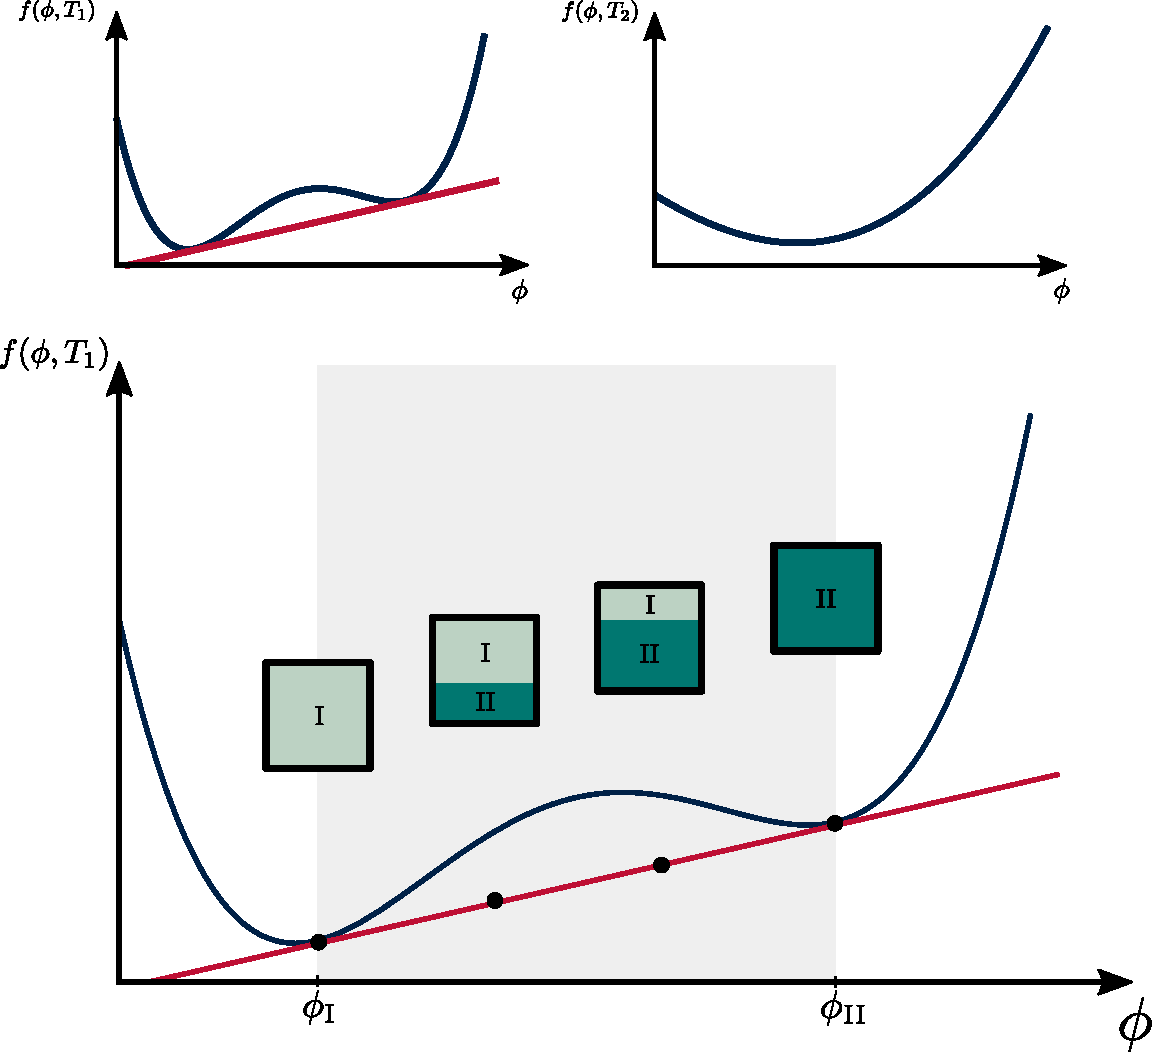
\includegraphics[width=\textwidth]{figures/thermo_solutions.pdf}
    \caption{Caption}
    \label{fig:phase_sep_scheme}
\end{figure}

Often, the shape of the free energy density can be controlled by some external parameter, such as temperature.

\todo{Comment on the energy barrier, spinodal binodal decomposition.}

\subsection{Regular Solution Model}
Mean field models of mixtures can describe the free energy density and predict features of the phase behaviour. The free energy density can be calculated from the Hamiltonian of a system and, again, the $A-B$ binary mixture is a useful place to start. Consider a lattice where each lattice site is occupied by either a molecule of $A$ or a molecule of $B$ where $v_A$ and $v_B$ (the size of each molecule) is the same and additionally define the total number of sites in the lattice $N_{lat} = N_A + N_B$. The different molecules can be configured in many different ways on the lattice however the different configurations will have different energies due to interactions between the molecules. The lattice model can include these interactions by having different contributions to the energy for different pairs of molecules on neighbouring lattice sites. For example, two molecules of $A$ on neighbouring sites will contribute $\epsilon_{AA}$ to the energy of a configuration, two molecules of $B$ contribute $\epsilon_{BB}$ and a molecule of $A$ on a neighbouring lattice site to a molecule of $B$ will contribute $\epsilon_{AB}$. The total energy of a configuration $c$ is then the sum of the interaction energy contribution over all neighbouring lattice sites
\begin{equation}
    E_{c} = N_c^{AA}\epsilon_{AA} + N_c^{AB}\epsilon_{AB} + N_c^{BB}\epsilon_{BB}
\end{equation}
where $N_c^{ij}$ is the number of neighbouring lattice sites, occupied by a molecule of $i$ and molecule of $j$ in the configuration. The free energy desnity can be calculated from the partition function, $Z$, where
\begin{equation}
    f(\phi, T) = -\frac{1}{\beta V}\ln Z
    \label{eq:f_ln}
\end{equation}
\todo{Put a KB T term into the new commands (and define it here)} and the partition function is directly calculated for a canonical ensemble via
\begin{equation}
    Z = \sum_c \exp{-\beta E_c}.
\end{equation}
where the sum is over all configurations. In the thermodynamic limit of large $N_{lat}$ the sum can be well approximated by a mean field approximation. The sum is approximated by replacing the energy of each configuration with the average energy, $\bar{E}$, so the sum now becomes
\begin{equation}
    Z \approx \sum_c \exp(-\beta \bar{E}) = \Omega \exp(-\beta \bar{E})
\end{equation}
where $\Omega$ is the number of unique configurations of molecules on the lattice and is given by
\begin{equation}
    \Omega = \frac{N_{lat}!}{N_A! N_B!}.
\end{equation}

The free energy density in the mean field model is now, with equation (\ref{eq:f_ln}), $f = -\frac{K_B T}{V} (\ln \Omega + \bar{E})$.

The mean energy $\bar{E}$ can be calculated ... The coordination number, $z$, describes the number of nearest neighbours each lattice site, for example $z=4$ in a square lattice. On average $z\phi_i$ of the neighbouring lattice sites will be occupied by a molecule of $i$. For $i \neq j$ the average number of $ij$ neighbour pairs, $\bar{N}^{ij}$, is the number of sites occupied by a molecule of $i$ multiplied by the average the number of neighbouring lattice sites occupied by a molecule of $j$: $\bar{N}^{ij} = N_{lat}\phi_i \times z\phi_j$. When $i=j$ each pair will be double counted (each lattice site occupied by a molecule of $i$ will be considered as both the `main' and `neighbour' site) and so there is an additional factor of 1/2 to prevent double counting. The average energy is therefore
\begin{equation}
\begin{split}
    \bar{E} &= \bar{N}^{AA}\epsilon_{AA} + \bar{N}^
    {AB}\epsilon_{AB} + \bar{N}^{BB}\epsilon_{BB}\\
    &= \frac{1}{2}z N_{lat} \phi^2\epsilon_{AA} + z N_{lat} (1-\phi)\phi\epsilon_{AB} + \frac{1}{2}z N_{lat} (1-\phi)^2 \epsilon_{BB}.
\end{split}
\end{equation}
Using equation (\ref{eq:f_ln}) the free energy density is
\begin{equation}
    f(\phi, T) = -\frac{1}{\beta V}\left(\ln \left(\frac{N_{lat}!}{N_A! N_B!} \right) - \frac{z N_{lat}}{2} \left(\phi^2\epsilon_{AA} + 2(1-\phi)\phi\epsilon_{AB} + (1-\phi)^2 \epsilon_{BB}\right)\right).
\end{equation}
The first term is simplified using Stirling's formula, $\ln N! = N \ln N - N$ for large $N$ to give $\ln\Omega=-N_{lat}(\phi\ln(\phi)+(1-\phi)\ln(1-\phi))$. The average energy term can be simplified as the phase behaviour described in \todo{section reference} was independent of the exact value of $f$, or $\partial f/\partial \phi$ and so the physics of the system is symmetric under a transform $f \rightarrow f + k_1 + k_2\phi$. Specifically, choosing $k_1 = z\epsilon_{BB}/2$ and $k_2 = z(\epsilon_{BB} - \epsilon_{AA})/2$ the free energy now becomes
\begin{equation}
    f(\phi, T) = k_B T (\phi\ln(\phi)+(1-\phi)\ln(1-\phi)) + \chi(1-\phi)\phi
\end{equation}
since $V = N_{lat}$ and define the Flory-Huggins interaction parameter $\chi = -\frac{z}{2 k_B T}(\epsilon_{AA}+\epsilon_{BB}-2\epsilon_{AB})$. \todo{Phase behaviour discussion for chi}

\todo{\begin{enumerate}
    \item Generalise to multi component
    \item Generalise to different volumes
    \item add in interface terms
    \item add in enthalpy terms
\end{enumerate}}
\begin{equation}
    f_{FH} = \sum_{i=1}^{N}\Bigg[\frac{\phi_i}{v_i}\ln\phi_i+\sum_{j=1, j\neq i}^{N}\frac{\chi_{ij}}{2}\phi_i\phi_j + \sum_{j=1}^{N} \frac{K_{ij}}{2}(\nabla\phi_i)\cdot(\nabla\phi_j)\Bigg]
    \label{fh_gen}
\end{equation}

where the scalars $\chi$ and $K$ now become $N \times N$ matrices describing the interactions between components and the surface tensions between domains of different compositions \cite{berry_physical_2018}. The constant number of lattice sites, $N_l$ naturally imposes incompressibility into the model ensuring that $\sum_{i=1}^N\phi_i=1$.
The Flory-Huggins model provides an extension to this regular solution model to reflect the different components as being molecules of different sizes. The model originally described polymers of chain length $N_P$ and introduced a correction to the entropic terms since the monomers on the chain are attached to each other which reduces the number of available configurations. We use this principle generally to extend the regular solution model in equation (\ref{rsm_gen}) to describe components of different size. This gives where $v_i$ describes the relative volumes of the components in the mixture. 

Another important contribution is from the intrinsic energy, the enthalpy, of each type of molecule which will appear proportionally to the number of molecules of that component in the system, $e_i \phi_i / v_i$. Previous work has often ignored this contribution as in a system of constant overall composition this term is simply an additive constant and so does not affect the behaviour of the solution. However the composition of a chemically active system can change and therefore this contribution may affect the system's behaviour.

The phase behaviour of these regular solution models is often dominated by the value of the interaction parameter, $\chi$. For $\chi > 0 $, there is an energetic cost to having different components mixing and can lead to phase separation. The interplay of entropic effects driving a homogeneous mixed state balanced against these additional terms determines the phase transitions. However all of these terms are derived from a free energy and provide an equilibrium description of the system. In fact, additional terms can be added to this equilibrium free energy density, such as terms from a generic external potential or higher order gradient terms. 

\section{Dynamics of Multi-component mixtures}

\subsection{Conserved Dynamics}

\todo{talk about the fact that $\phi$ can vary spatially?}

\subsubsection{Model B Dynamics}
\todo{Physics of active emulsions is quite a good reference for this.}
\todo{Linear response model?}
\todo{Comment on non momentum conservation}
The static lattice picture can describe the free energy of a system, but fails to capture associated dynamics. The lattice model can be extended to include the evolution of a system through configuration space by considering exchange of molecules of neighbouring lattice sites. In this picture (and also physically), the number of molecules of each species does not change and so the behaviour of the volume fraction for each component must obey a continuity equation, namely\cite{li_non-equilibrium_2020}
\begin{equation}
    \dot{\phi}_i = - \nabla \cdot \textbf{J}_i
    \label{eq:continuityModB}
\end{equation}
\todo{keep track of KB Ts} where $i$ labels each component, and $\textbf{J}_i$ is the volume fraction flux. \todo{Tidy the following up. Is Model B phenomenological?} Changes to the distribution of a component will be driven by changes in the free energy and specifically, the associated thermodynamic force, the chemical potential. The canonical Model B dynamics capture this chemical pressure and give the volume fraction flux as
\begin{equation}
    \textbf{J}_i = \sum_j M_{ij}\nabla\mu_j + \textbf{J}^N
    \label{eq:fluxModB}
\end{equation}
where $\mu_i$ is the chemical potential of the $i\th$ component, $M_{ij}$ is a set of generalised mobilities (discussed in the \todo{next section}) and the sum runs over all components in the system. The $\textbf{J}^N$ term describes the noise and must obey the appropriate fluctuation dissipation theorems. In the thermodynamic limit of a noise free model considered here the $ \textbf{J}^N$ contribution vanishes. The chemical potential for each component, $\mu_i$, is given by
\begin{equation}
    \mu_i = v_i\frac{\delta F}{\delta \phi_i}.
\end{equation}
where the additional volume term compared to equation (\ref{eq:mu_def}) is due to the conversion from particle number to volume fraction \todo{clarify this and fit in with the other}.

\subsubsection{Mobilities for Incompressible Models}
\todo{Mazur and de Groot reference?}
The model B dynamics introduce a set of transport coefficients, or mobilities $M_{ij}$, which describe how volume fraction of the $i\th$ component responds to the chemical potential of the $j\th$ component. This is a general form of linear transport relationship found near equilibrium in thermodynamic systems where the flux is proportional $J_i = \sum_{j}L_{ij}\nabla f_{j}$ where the thermodynamic forces are conjugate to the displacements being described. In this generalised description, the transport coefficient matrix described by $L_{ij}$ is both positive semi-definite (positive entropy production rate) and symmetric under exchange of $i, j \rightarrow j, i$. Here however, the flux describes the transport of volume fraction rather than particle number and so the the forces and displacements are not conjugate. As such the reciprocity is broken and $L_{ij} \neq L_{ji}$, however again using the size of individual molecules to convert between volume fraction and number density gives
\begin{equation}
    {M}_{ij} = \frac{v_i}{v_j}{M}_{ji}.
    \label{eq:mobsym}
\end{equation}

The lattice model is incompressible when the total number of lattice sites, $N_{lat}$, is constant. The incompressibility condition can be written as $\sum_i\phi_i = 1$ and so $\sum_i\dot{\phi}_i = 0$. Substituting in the Model B dynamics, equations (\ref{eq:continuityModB}) and (\ref{eq:fluxModB}) give
\begin{equation}
    \sum_i\dot{\phi}_i = \sum_i\;\nabla\cdot\bigg(\sum_j M_{ij}\nabla\mu_j\bigg) = \sum_j\;\nabla\cdot\bigg(\big(\sum_i M_{ij}\big)\nabla\mu_j\bigg) = 0
\end{equation}
In order for this to be true in general, for non-uniform systems, i.e. $\nabla\mu_j \neq 0$, it is necessary for the mobilities to satisfy
\begin{equation}
    \sum_i M_{ij} = 0
    \label{eq:mobinc}
\end{equation}
which constrains the mobilities and enforces the fluid remains incompressible.\cite{kehr_mobility_1989} An $N$-component mixture,  has a total of $N\times N$ mobilities. The reciprocity-like constraint in equation (\ref{eq:mobsym}) reduces the number of free parameters to $N(N+1)/2$ and the incompressibility condition adds a further $N$ constraints to give $N(N-1)/2$ free mobility parameters.

\subsection{Non-Conserved Dynamics}

\subsubsection{Reaction Rates}
In addition to spatial fluxes of component from the Model B dynamics, chemically active mixtures will also permit fluxes in chemical space, i.e. the conversion of a molecule of $i$ to a molecule of $j$. Putting these dynamics into the binary mixture, we allow the reaction $A \rightleftharpoons B$, and an immediate consequence of incompressibility is that the reaction must conserve volume, so here $v_A = v_B$. In general the volume of the reactants must equal the volume of the products which is simple for this 1:1 stoichiometry but could be more complex for non-conserved molecule number. The change in the free energy due to the reaction is $dF = \mu_A dN_A+\mu_B dN_B = (\mu_A - \mu_B)dN_A$ where $dN_A = -dN_B$ by conservation of total molecule number. There is therefore no net conversation between molecules of $A$ and $B$ when $\mu_A = \mu_B$ and \todo{justify/explain this} the rate of the reaction is given by... Considering detailed balance for the system constrains the relationship between the forward and backward reaction rates
\begin{equation}
    \frac{r_{A \rightarrow B}}{r_{B \rightarrow A}} = \exp\Bigg(\frac{\mu_A - \mu_B}{k_B T}\Bigg)
    \label{db_constr}
\end{equation}
which allows us to identify the net transfer from $A \rightarrow B$ as
\begin{equation}
    r_{A \rightarrow B} - r_{B \rightarrow A} = K\Bigg(\exp\bigg(\frac{\mu_A - \mu_B}{k_B T}\bigg)-1\Bigg)
    \label{eq:sponrate}
\end{equation}
which makes sense as if $\mu_A > \mu_B$ then we have net $A \rightarrow B$, when $\mu_B > \mu_A$ then we have net $B \rightarrow A$ and at equilibrium $\mu_A = \mu_B$\cite{weber2019physics}.
\todo{Example of how this reduces to mas action}

\subsubsection{Enzymatic Activity}
Enzymes act as catalysts in biological reactions and increase the rate of a reaction. This can be achieved by the presence of an active site that allows the reaction to occur or via some alternative reaction route    fuel driven reaction that occurs only in the presence of this \textit{enzyme} component. The reaction that now occurs is
\begin{equation}
    \text{Enzyme + Fuel} + A \leftrightharpoons \text{Enzyme + Waste} + B
\end{equation}
where the system is in contact with a Fuel and Waste reservoir that maintains constant chemical potentials, $\mu_{Fuel}$ and $\mu_{Waste}$ and define $\Delta\mu \equiv \mu_{Fuel}-\mu_{Waste}$ which is also constant. Alternatively, $\Delta \mu$ could represent the energy transferred by a photon in a light-activated catalytic reaction. Using equation (\ref{db_constr}) the rate of $A \rightarrow B$ of this reaction in the presence of the enzyme can be written as
\begin{equation}
    r_{A \rightarrow B,E} - r_{B \rightarrow A,E} = K'\rho_\textrm{E}\Bigg(\exp\bigg(\frac{\mu_A - \mu_B + \Delta\mu}{k_B T}\bigg)-1\Bigg)
    \label{eq:enzrate}
\end{equation}
where the reaction rate is proportional to the local concentration of the enzyme component, $\rho_\textrm{E}$ and $K'$ is the modified rate constant. Reaction kinetics of enzymes are often described using Michaelis–Menten kinetics where $r_{A\rightarrow B}\sim\rho_\textrm{E}\rho_\textrm{A}/(K_{M}+\rho_\textrm{A})$ where $K_M$ is the Michaelis constant and $\rho_\textrm{A}$ is the concentration of the substrate, A\cite{murray_mathematical_1993}. In both  descriptions of the kinetics, the rate increases linearly with $\rho_\textrm{E}$ however, equation (\ref{eq:enzrate}) will additionally capture the effect of interactions on the rate of conversion when compared to the Michalis-Menten rate.

\section{Minimal Model of an Active Mixture}

The simplest model that will encapsulate all of these effects requires at least two components for a chemical reaction to occur, e.g. $S \rightleftharpoons P$ (substrate to product) and a third enzyme component (E), that permits the driven, catalytic reaction described in equation (\ref{eq:enz_rates}). At every point in space and time system is parameterised by three volume fractions; $\phis(\bm{r},t)$, $\phip(\bm{r},t)$ and $\phie(\bm{r},t)$, corresponding to individual molecules of volume $\vs$, $\vp$ and $\ve$ respectively. The mixture is incompressible and so $\phis+\phip+\phie=1$ everywhere and consequently the reaction requires, $\vs = \vp$. In living systems, enzymes have much more complex structures than reactants and so we expect the size of this component to be much larger $\ve > \vs, \vp$\cite{berg_biochemistry_2002}. This increased size is also expected to result in increased viscous drag and reduced mobility for an enzyme compared to the other components. The Flory-Huggins theory of suspensions gives the free energy of the system as $F = \int \mathrm{d}\bm{r} f_\mathrm{FH}$, with the free energy density
\begin{equation}
    f_\mathrm{FH}(\{\phi_i\}) = \sum_{i=1}^{N} \frac{1}{v_i} \big[\varepsilon_i\phi_i + k_\mathrm{B}T \phi_i \big(\log\phi_i-1\big) \big], 
    \label{eq:fh_gen}
\end{equation}
where $\varepsilon_i$ is the enthalpy of component $i$. Importantly, we do not include any interaction terms in the free energy, in particular $f_\mathrm{FH}$ does not contain terms of the usual form $\chi_{ij}\phi_i \phi_j$. This implies that phase separation in this system would be impossible at equilibrium. The chemical potential of a component is given by
\begin{equation}
    \mu_i = e_i + \log\phi_i + 1 \quad \text{and so} \quad \nabla\mu_i = \frac{1}{\phi_i}\nabla\phi_i
    \label{eq:chempot}
\end{equation}
which drive the conserved dynamics of Model B. Fo the mobilities we assume the common form where $M_{ij} = -\beta D_{ij}\phi_i\phi_j$ for $i \neq j$ and $\beta \equiv (k_\mathrm{B}T)^{-1}$. The mobility constraints imply $M_{jj}= - \sum_{i\neq j} M_{ij}$ and $v_j D_{ij} = v_i D_{ji}$ \cite{KRAMER1984473, kehr_mobility_1989, mao_designing_2020, bo_stochastic_2021}. The transport coefficients $D_{ij}$ determine the rate at which the components respond to local effective concentration gradients and exchange positions, and as such are inherently related to the phenomena of diffusiophoresis, cross-diffusion and Maxwell-Stefan diffusion \cite{suppmat}.

We make the model active by allowing non-equilibrium (fuelled) conversion between two components, substrate (S) and product (P), catalyzed by an enzyme (E). This can be described by the reaction E+S+F $\rightleftharpoons$ E+P+W, where F and W represent fuel and waste molecules, respectively. We do not model the dynamics of the fuel and waste here, but assume that the system is in contact with a reservoir that maintains constant chemical potentials, $\muf$ and $\muw$, and define $\Delta\mu \equiv \muf-\muw$. The catalysed reaction converts substrate to product with rate $\rcat$ and we also model the spontaneous reaction (does not require enzyme) which converts substrate to product at rate $\rspo$ (note that these contributions might be negative as this flux is always expressed in the direction $S \rightarrow P$). Evaluating equations (\ref{eq:sponrate}) and (\ref{eq:enzrate}) with the chemical potential from equation (\ref{eq:chempot}) gives
\begin{align}
    \rspo &= \rspo^{\mathrm{S}\to\mathrm{P}} - \rspo^{\mathrm{P}\to\mathrm{S}} = \kspo[e^{\beta \Delta \varepsilon}\phis - \phip],\\
    \rcat &= \rcat^{\mathrm{S}\to\mathrm{P}} - \rcat^{\mathrm{P}\to\mathrm{S}} = \kcat\phie[\phis-\phip e^{-\beta(\Delta \varepsilon+ \Delta\mu)}],
    \label{r_cat}
\end{align}
where $\Delta e = e_S - e_P$. The rate constants here have been scaled to better disentangle the effects of the various parameters; $k_{spo} = K_{spo}/\phi_P$ and $k_{cat} = K_{cat}e^{-(\Delta e + \Delta \mu)}/(\ve \phi_P)$. We will typically take $\Delta \varepsilon<0$ and $\Delta \varepsilon + \Delta \mu>0$, so that the spontaneous and catalyzed reactions run preferentially in the P$\to$S and S$\to$P directions, respectively; see Fig.~\ref{fig:cartoon-schematic}.

Combining the conserved and non-conserved dynamics and defining $R\equiv\rspo+\rcat$ results in the evolution equations for the three-component system
\begin{align}
    \dot{\phie} &= \bm{\nabla} \cdot \big(\Mee\bm{\nabla}\mue + \Mes\bm{\nabla}\mus + \Mep\bm{\nabla}\mup\big), \label{evoE}\\
    \dot{\phis} &= \bm{\nabla} \cdot \big(\Mse\bm{\nabla}\mue + \Mss\bm{\nabla}\mus + \Msp\bm{\nabla}\mup\big) - R, \label{evoS}\\
    \dot{\phip} &= \bm{\nabla} \cdot \big(\Mpe\bm{\nabla}\mue + \Mps\bm{\nabla}\mus + \Mpp\bm{\nabla}\mup\big) + R. \label{evoP}
\end{align}

\section{Catalysis Induced Phase Separation}
\subsection{Stability of the Homogeneous Steady State}
The minimal active mixture described by equations (\ref{evoE})-(\ref{evoP}) can be seen to have a uniform steady state solution when $R=0$. All other terms describing the evolution from gradients in the chemical potentials vanish for a homogeneous system and solving for $R=0$ yields the stationary state with
\begin{align}
    \phi_S^* = \alpha\frac{(k_{cat}\phi_E^*-k_{spo})}{k_{cat}\phi_E^*(e^{\Delta e + \Delta\mu}+1) - k_{spo}(\text{exp} (\Delta e)+1)} \label{sstar}
    \\
    \phi_P^* = \alpha\frac{(k_{cat}\phi_E^*\text{exp} (\Delta e + \Delta\mu) - k_{spo}(\text{exp} (\Delta e))}{k_{cat}\phi_E^*(\text{exp} (\Delta e + \Delta\mu)+1) - k_{spo}\text{exp} (\Delta e+1)} 
    \label{pstar}
\end{align}
where the star indicates that these quantities are at $R=0$ and $\alpha$ is the total amount of product and substrate in the system $\alpha = \phi_S^*+\phi_P^*$ and for the minimal mixture case, $\alpha = 1-\phi_E^*$. We consider a small perturbation from this uniform steady state $\phi_i \rightarrow \phi_i^* + \delta\phi_i$ giving $\mu_i \rightarrow \mu_i^* + \delta\mu_i$. Equation (\ref{chempots}) gives $\delta\mu = \frac{\delta\phi_i}{\phi_i^*}$ and so $\nabla\mu_i = \frac{1}{\phi_i^*}\nabla\delta\phi_i$ (both to first order) and also define $M^*_{ij} = M_{ij}(\phi_E^*, \phi_S^*, \phi_P^*)$. Finally, expand $R$ around the $R=0$ solution, to give $\delta R = R_E\delta\phi_E+R_S\delta\phi_S-R_P\delta\phi_P$ (where the signs are chosen such that all $R_i \geq 0$).
\begin{align}
    R_E &= k_{cat}[\phi_S^*-\phi_P^*e^{(\Delta e + \Delta \mu)}] = \alpha\frac{k_{cat}k_{spo}(1-e^{\Delta \mu})}{k_{spo}+k_{cat}\phi_E^*e^{-(\Delta e + \Delta \mu)}+k_{spo}e^{\Delta e}+k_{cat}\phi_E^*}\\
    R_S &= k_{spo}e^{\Delta e} + k_{cat}\phi_E^*\\
    R_P &= k_{spo} + k_{cat}\phi_E^*e^{-(\Delta e+\Delta \mu)}
\end{align}

We consider perturbations from this steady state of the form $\delta\phi_i = |\delta\phi_i| e^{i\textbf{q}\cdot\textbf{r}}$ and the resulting linear response of the system can be written as

\noindent
\makebox[\textwidth]{\parbox{1.3\textwidth}{%
\begin{equation}
\begin{pmatrix}
\dot{\delta\phi_E}\\
\dot{\delta\phi_S}\\
\dot{\delta\phi_P}\\
\end{pmatrix} =
\underbrace{
\begin{pmatrix}
(M_{SE}^*+M_{PE}^*)\frac{\textbf{q}^2}{\phi_E^*} & -M_{SE}^*\frac{v_E}{v_S}\frac{\textbf{q}^2}{\phi_S^*} & -M_{PE}^*\frac{v_E}{v_P}\frac{\textbf{q}^2}{\phi_P^*}\\
-M_{SE}^*\frac{\textbf{q}^2}{\phi_E^*} - R_E & \big(M_{SP}^* + M_{SE}^*\frac{v_E}{v_S}\big)\frac{\textbf{q}^2}{\phi_S^*} - R_S & -M_{SP}^*\frac{\textbf{q}^2}{\phi_P^*} + R_P\\
-M_{PE}^*\frac{\textbf{q}^2}{\phi_E^*}  + R_E & -M_{SP}^*\frac{\textbf{q}^2}{\phi_S^*} + R_S & \big(M_{PE}^*\frac{v_E}{v_P}+M_{SP}^*\big)\frac{\textbf{q}^2}{\phi_P^*} - R_P\\
\end{pmatrix}
}_{C}
\begin{pmatrix}
\delta\phi_E\\
\delta\phi_S\\
\delta\phi_P\\
\end{pmatrix}
\end{equation}}}
where we can explicitly see the incompressibility being imposed as the columns of $C$ sum to zero
\begin{equation}
    \sum_i\dot{\delta\phi_i} = \sum_{i,j}C_{ij}\delta\phi_j = \sum_{j}0\times\delta\phi_j = 0
\end{equation}
which allows one of the components to be eliminated. As an example, set $\delta\phi_P = -\delta\phi_E - \delta\phi_S$ and thus we can define a $2\times2$ matrix, $C'$ describing the evolution where we subtract the last column of the other two, i.e. $C'_{ij} = C_{ij} - C_{i3}$ for $i, j \in {1, 2}$, giving
\noindent
\makebox[\textwidth]{\parbox{1.3\textwidth}{%
\begin{equation}
\begin{pmatrix}
\dot{\delta\phi_E}\\
\dot{\delta\phi_S}\\
\end{pmatrix} =
\underbrace{
\begin{pmatrix}
(M_{SE}^*+M_{PE}^*)\frac{\textbf{q}^2}{\phi_E^*} +M_{PE}^*\frac{v_E}{v_P}\frac{\textbf{q}^2}{\phi_P^*}& -M_{SE}^*\frac{v_E}{v_S}\frac{\textbf{q}^2}{\phi_S^*} + M_{PE}^*\frac{v_E}{v_P}\frac{\textbf{q}^2}{\phi_P^*}\\
-M_{SE}^*\frac{\textbf{q}^2}{\phi_E^*} - R_E + M_{SP}^*\frac{\textbf{q}^2}{\phi_P^*} - R_P & \big(M_{SP}^* + M_{SE}^*\frac{v_E}{v_S}\big)\frac{\textbf{q}^2}{\phi_S^*} - R_S + M_{SP}^*\frac{\textbf{q}^2}{\phi_P^*} - R_P\\
\end{pmatrix}
}_{C'}
\begin{pmatrix}
\delta\phi_E\\
\delta\phi_S\\
\end{pmatrix}
\end{equation}}}
The eigenvalues of $C'$ determine the stability of the steady state. The system is stable if and only if all of $C'$'s eigenvalues are negative. Since $C'_{1,1}$ and $C'_{2,2}$ are always negative (from the Onsager constraints and the non-negativity of $R_i$), $\text{tr}(C') < 0$ and there is therefore one positive eigenvalue if $\det(C')<0$. The instability condition then becomes
\begin{equation}
\begin{split}
    \Bigg((M_{SE}^*+M_{PE}^*)&\frac{\textbf{q}^2}{\phi_E^*} + M_{PE}^*\frac{v_E}{v_P}\frac{\textbf{q}^2}{\phi_P^*}\Bigg)\Bigg(\big(M_{SP}^* + M_{SE}^*\frac{v_E}{v_S}\big)\frac{\textbf{q}^2}{\phi_S^*} - R_S + M_{SP}^*\frac{\textbf{q}^2}{\phi_P^*} - R_P\Bigg) \\
    &< \Bigg(-M_{SE}^*\frac{v_E}{v_S}\frac{\textbf{q}^2}{\phi_S^*} + M_{PE}^*\frac{v_E}{v_P}\frac{\textbf{q}^2}{\phi_P^*}\Bigg)\Bigg(-M_{SE}^*\frac{\textbf{q}^2}{\phi_E^*} - R_E + M_{SP}^*\frac{\textbf{q}^2}{\phi_P^*} - R_P\Bigg)
\end{split}
\label{hi_ord_ins}
\end{equation}
For very large values of $\textbf{q}$, we expect the system to be stable as in this regime the evolution is dominated by diffusive effects. When $\textbf{q} \rightarrow 0$ the system should be at the critical stability as this corresponds to a uniform change in the $\phi_i$s. As such, since this condition only depends on $\textbf{q}^2$ and $\textbf{q}^4$ the instability is satisfied if and only if it is satisfied for very small $\textbf{q}^2$. With this is mind we take equation (\ref{hi_ord_ins}) to first order in $\textbf{q}^2$ which gives
\begin{align}
    \frac{1}{v_E\phi_E^*}+\frac{1}{v_P(1-\phi_E^*)} < \frac{R_E}{v_P(1-\phi_E^*)}\bigg(\frac{\gamma_P}{R_S}-\frac{\gamma_S}{R_P}\bigg)
    \label{eq_form_cond}
\end{align}
where we have defined
\begin{equation}
    \gamma_S \equiv \frac{M_{SE}^*}{M_{SE}^*+M_{PE}^*} \quad \text{   and    } \quad \gamma_P \equiv \frac{M_{PE}^*}{M_{SE}^*+M_{PE}^*}
\end{equation}
Remembering that $R_E \propto (e^{\Delta\mu} - 1)$ we see that for $\Delta\mu=0$, $R_E = 0$ and the instability cannot be satisfied at equilibrium. This condition can also be written to constrain the relative volumes in the system
\begin{equation}
    \frac{v_P}{v_E} < \frac{\phi_E^*}{1-\phi_E^*}\Bigg(R_E\bigg(\frac{\gamma_P}{R_S}-\frac{\gamma_S}{R_P}\bigg) - 1\Bigg)
    \label{vol_ins}
\end{equation}
We can assume a form for $M_{SE} = -D_{SE}\phi_E\phi_S$ and $M_{PE} = -D_{PE}\phi_E\phi_P$ which results in
\begin{equation}
    \frac{1}{v_E\phi_E^*}+\frac{1}{v_P(1-\phi_E^*)} < \frac{R_E}{v_P(1-\phi_E^*)}\frac{D_{PE}-D_{SE}}{D_{PE}R_S+D_{SE}R_P}
\end{equation}
\begin{equation}
\begin{split}
\text{RHS} &= \frac{k_{cat}k_{spo}(1-e^{-\Delta\mu})}{v_P(k_{spo}+k_{cat}\phi_E^*e^{-(\Delta e+\Delta\mu)}+k_{spo}e^{\Delta e}+k_{cat}\phi_E^*)} \\ 
& \quad \quad \times \frac{D_{PE}-D_{SE}}{D_{PE}(k_{spo}e^{\Delta e}+k_{cat}\phi_E^*)+D_{SE}(k_{spo}+k_{cat}\phi_E^*e^{-(\Delta e+\Delta\mu)})}
\end{split}
\end{equation}
In calculating this condition we eliminated the product component from the system and determined the stability from considering the other two components. Alternatively, we could have eliminated either of the other components and require the same negative eigenvalues stability condition, which give the same result. A quick check for eliminating the substrate instead can be seen by noticing the expression is invariant under $S, P \rightarrow P, S$ and $R_E \rightarrow -R_E$, which is the same difference between the second and third rows of $C'$. Prior work often imposes incompressibility by eliminating one of the components and using $\phi_i = 1-\sum_{j,j\neqi}\phi_j$. This can be an effective equilibrium description, but when the approach to equilibrium and dynamics and considered, the correct choices for mobilities must also be constructed to impose the incompressibility naturally.

Larger $D_{PE}-D_{SE}$ makes the system more unstable. This can be understood, as $D_{PE}$ is a measure of how quickly the product component moves to regions of higher enzyme concentration. Since the enzyme allows for more product, this creates a feedback where the product moves to product faster than the substrate and this makes the system unstable. This preferential attraction must overcome the diffusive behaviour of the system to drive the instability. Equation (\ref{vol_ins}) also shows the stability depends on the ratio of $\frac{v_S}{v_E}$. The system is more unstable for much larger enzyme sizes compared to the substrate and product which is a convenient result since, as previously discussed, enzymes are often significantly larger than the substrate or products involved in the corresponding reaction. A similar size dependence can be seen in colloidal systems. Depletion forces arise from a particle of  intermediate size (between the size of the solvent and colloids) having an increased available volume to occupy when the colloids aggregate, even from simple hard sphere interactions. As a consequence there is an osmotic pressure driving this aggregation of the colloids\cite{jones2002soft}. In this system, it is less obvious how aggregation will increase the volume for the components to occupy and it is unclear how similar the effect would be to these depletion interactions. Additionally, we only have two particle sizes in this model with no intermediate size and hard sphere interactions are not modelled within the lattice framework that motivated the form of the free energy, equation (\ref{f}). The volume terms in the free energy cancel when deriving the evolution equations for the system, equations (\ref{evoE}) to (\ref{evoP}), and only appear as a consequence of the forms of the mobility, potentially suggesting another size dependent mechanism for the instability.

\subsection{Stability of a Multi-Component Non-Interacting System}

Equation (\ref{eq_form_cond}) shows that for the minimal model the equilibrium system, $\Delta\mu=0$, is stable. It can also be shown that a general $N$-component incompressible fluid without chemical interactions is stable. We assume that the chemical potentials follow a non-interacting Flory-Huggins free energy (equation (\ref{chempots})) and assume Model B noise free dynamics, we find perturbations around the uniform steady state (the $*$ state) to behave as

\begin{equation}
    \dot{\delta\phi_i} = \sum_j M_{ij}^*\frac{\nabla^2\delta\phi_j}{\phi_j^*} = \sum_j\Bigg( M_{ij}^*\frac{1}{\phi_j^*}\times-\textbf{q}^2\delta\phi_j\Bigg)
\end{equation}
where we consider perturbations of the form $\delta\phi_i = |\delta\phi_i|e^{i\textbf{q}\cdot \textbf{r}}$. This system can be described considering the vector of perturbations $\overrightarrow{\delta\phi}=(\delta\phi_1, \delta\phi_2, ..., \delta\phi_N)^T$ to give
\begin{equation}
    \dot{\overrightarrow{\delta\phi}} &=-\textbf{q}^2 \underbrace{\text{diag}\big(v_1, ..., v_N\big)}_{\hat{v}}\:\widetilde{M}\: \underbrace{\text{diag}\big(\phi_1^{-1}, ..., \phi_N^{-1}\big)}_{\hat{G}}\overrightarrow{\delta\phi}
\end{equation}
where $\widetilde{M}$ is known to be positive semi-definite from Onsager reciprocal relations and we have defined $\hat{v} = \text{diag}(v_1, v_2, ...v_N)$ and $\hat{G} = \text{diag}(\phi_1^{-1}, ..., \phi_N^{-1})$. This system is not unstable if and only if all of the eigenvalues of the matrix $\hat{v}\widetilde{M}\hat{G}$ are non-negative, which is equivalent to $\textbf{x}^T\hat{v}\widetilde{M}\hat{G}\textbf{x} \geq 0$ and $\textbf{x}^T\hat{G}\widetilde{M}\hat{v}\textbf{x} \geq 0$ since $\hat{G}$, $\widetilde{M}$, and $\hat{v}$ are symmetric. Summing these conditions gives $\textbf{x}^T(\hat{G}+\hat{v})\widetilde{M}(\hat{G}+\hat{v})\textbf{x} \geq 0$ where we note that $(\hat{G}+\hat{v})$ is a diagonal matrix with positive, non-zero entries along the diagonal. Since $\widetilde{M}$ is positive semidefinite, the product will also be positive semi-definite and so the system is linearly stable to all perturbations around this uniform steady state.

\subsection{Fast Dynamics}
In deriving the stability condition for the minimal active mixture, we note that the eigenvalues of a $2\times2$ matrix can be given in terms of its trace, $T$ and determinant, $D$, as $\lambda_{\pm} = \frac{1}{2}(T \pm \sqrt{T+4D})$. Alternatively we can make the assumption of fast substrate and product dynamics in comparison to the enzyme dynamics. Since the enzymes are expected to be much larger than the product and substrate, we expect that they may also move much slower and that the product and substrate equilibrate much more quickly. This suggest we can write $\dot{\delta\phi_S}=0$ and thus we find a relationship between  $\delta\phi_S$ and $\delta\phi_E$. This gives 
\begin{equation}
    \dot{\delta\phi_S} &= C'_{21}\delta\phi_E + C'_{22}\delta\phi_S = 0 \implies \delta\phi_S &= -\frac{C'_{21}}{C'_{22}}\delta\phi_E \implies \dot{\delta\phi_E} = C'_{11}\delta\phi_E  - C'_{12}\frac{C'_{21}}{C'_{22}}\delta\phi_E
\end{equation}
and the instability condition then becomes
\begin{equation}As an example we consider the three component (E, S, P), minimal active mixture. Due to the incompressibility condition, we have $v_S=v_P$ and so we can write the mobility matrix as
\begin{equation}
M = 
\begin{pmatrix}
M_{EE} & M_{ES} & M_{EP}\\
M_{SE} & M_{SS} & M_{SP}\\
M_{PE} & M_{PS} & M_{PP}\\
\end{pmatrix}
=
\begin{pmatrix}
-(M_{SE}+M_{PE}) & M_{SE}\frac{v_E}{v_S} & M_{PE}\frac{v_E}{v_P}\\
M_{SE} & -(M_{SE}\frac{v_E}{v_S}+M_{SP}) & M_{SP}\\
M_{PE} & M_{SP} & -(M_{PE}\frac{v_E}{v_P}+M_{SP})\\
\end{pmatrix}
\label{ESP_mob}
\end{equation}
The free mobilities to be defined here are $M_{SE}$, $M_{PE}$, and $M_{SP}$, which in general can be a function of $\phi_E$, $\phi_S$, and $\phi_P$.


which we can find directly for a non interacting system described by equation (\ref{f}) to be
\begin{equation}
    \mu_i = e_i + \log\phi_i + 1 \quad \text{and so} \quad \nabla\mu_i = \frac{1}{\phi_i}\nabla\phi_i.
    \label{chempots}
\end{equation}

    C'_{11} - C'_{12}\frac{C'_{21}}{C'_{22}} > 0.
\end{equation}
Looking at the form of $C'_{22}$, in the small $\textbf{q}$ limit, $C'_{22}=-(R_S+R_P) < 0 $, which gives
\begin{equation}
    C'_{11}C'_{22}&-C'_{21}C'_{12} < 0 \\
\end{equation}
which is that $\det[C'] < 0$ as noted before by considering the eigenvalues. We subsequently use this slow enzyme assumption when dealing with enzymes and other interacting, fast components.
\subsection{Wet System}
An additional solvent component (e.g. water) can be added to the system similarly to the other components, with no reaction terms. Following a similar procedure as for the dry (no solvent) case, we can expand around a steady state where we now have $\alpha \neq 1 - \phi^*_E$ but $\phi_W^* = 1 - \alpha - \phi^*_E$. We can eliminate the solvent volume fraction to give a $3\times3$ matrix describing the evolution of E, S, and P volume fractions; $(\dot{\delta\phi_E}, \dot{\delta\phi_S}, \dot{\delta\phi_P})^T = C'_W(\delta\phi_E, \delta\phi_S, \delta\phi_P)^T$ with
\noindent
\makebox[\textwidth]{\parbox{1.3\textwidth}{%
\begin{equation}
    C_W = 
\begin{tiny}
\begin{pmatrix}
(M_{SE}^*+M_{PE}^*+M_{WE}^*)\frac{\textbf{q}^2}{\phi_E^*}+M_{WE}^*\frac{v_E}{v_W}\frac{\textbf{q}^2}{\phi_W^*} & -M_{SE}^*\frac{v_E}{v_S}\frac{\textbf{q}^2}{\phi_S^*}+M_{WE}^*\frac{v_E}{v_W}\frac{\textbf{q}^2}{\phi_W^*} & -M_{PE}^*\frac{v_E}{v_P}\frac{\textbf{q}^2}{\phi_P^*}+M_{WE}^*\frac{v_E}{v_W}\frac{\textbf{q}^2}{\phi_W^*}\\
-M_{SE}^*\frac{\textbf{q}^2}{\phi_E^*}-R_E+M_{WS}^*\frac{v_S}{v_W}\frac{\textbf{q}^2}{\phi_W^*} & (M_{SE}^*\frac{v_E}{v_S}+M_{SP}^*+M_{WS}^*)\frac{\textbf{q}^2}{\phi_S^*}-R_S +M_{WS}^*\frac{v_S}{v_W}\frac{\textbf{q}^2}{\phi_W^*}& -M_{SP}^*\frac{\textbf{q}^2}{\phi_P^*}+R_P+M_{WS}^*\frac{v_S}{v_W}\frac{\textbf{q}^2}{\phi_W^*}\\
-M_{PE}^*\frac{\textbf{q}^2}{\phi_E^*}+R_E+M_{WP}^*\frac{v_P}{v_W}\frac{\textbf{q}^2}{\phi_W^*} & -M_{SP}^*\frac{\textbf{q}^2}{\phi_S^*}+R_S+M_{WP}^*\frac{v_P}{v_W}\frac{\textbf{q}^2}{\phi_W^*} & (M_{PE}^*\frac{v_E}{v_P}+M_{SP}^*+M_{WP}^*)\frac{\textbf{q}^2}{\phi_P^*}-R_P+M_{WP}^*\frac{v_P}{v_W}\frac{\textbf{q}^2}{\phi_W^*}\\
\end{pmatrix}
\end{tiny}
\end{equation}
}}

We again can assume that the substrate and product dynamics are fast in comparison to the enzyme. Setting $\dot{\delta\phi_S}=\dot{\delta\phi_P}=0$ gives
\begin{equation}
    \dot{\delta\phi_E} = (C'_W^{-1})_{1, 1}\delta\phi_E
\end{equation}
and so the stability condition becomes
\begin{equation}
    (C'_W^{-1})_{1, 1} = \frac{(C'_W)_{2, 2}(C'_W)_{3, 3}-(C'_W)_{2, 3}(C'_W)_{3, 2}}{\det(C'_W)} \geq 0
    \label{solvstab}
\end{equation}
The numerator of equation (\ref{solvstab}) is, to order $\textbf{q}^2$
\begin{equation}
    \textbf{q}^2\Bigg[-R_P\frac{M_{SE}^*\frac{V_E}{V_S}+M_{WS}^*}{\phi_S^*}-R_S\frac{M_{PE}^*\frac{V_E}{V_S}+M_{WP}^*}{\phi_P^*}-\frac{v_P}{v_W\phi_W^*}\big(R_S+R_P\big)\big(M_{WS}^*+M_{WP}^*\big)\Bigg]
    \label{solvnum}
\end{equation}
We know that $(M_{SE}+M_{PE}+M_{WE})<0$ from the Onsager positivity conditions and for the common choice of mobilities, $M_{ij}<0$ for $i \neq j$. Therefore, we assume that expression (\ref{solvnum}) is positive and that stability is determined simply by the sign of the determinant. An equivalent interpretation is that we naturally have all negative eigenvalues and thus a negative determinant changing sign when one of the eigenvalues changes sign, since the determinant is equal to the product of the eigenvalues.

The determinant of $C_W'$ has many terms and even when truncated to order $\textbf{q}^2$ it is not obvious how to interpret the resulting expression. A particular observation is that in the low/no solvent limit ($\frac{1}{\phi_W}$ is very large) and assuming the $M_{ij}$s are the same size we get

\begin{equation}
\begin{split}
    \det(C'_W) &= M_{PE}^*\phi_SM'_W\big(\phi_E(R_E-R_S)\frac{v_E}{v_P}-\phi_P(R_P+R_S)\big)  \\
    &- M_{SE}^*\phi_PM'_W\big(\phi_E(R_E+R_P)\frac{v_E}{v_P}+\phi_S(R_P+R_S)\big) \\
    &- M_{WE}^*\Bigg(M_{WP}^*\phi_S\big(\phi_E(-R_E+R_S)\frac{v_E}{v_P}+\phi_P(R_P+R_S)) \\
    &+M_{WS}^*\phi_P\big(\phi_E(R_E+R_P)\frac{v_E}{v_P}+\phi_S(R_P+R_S))\Bigg)
\end{split}
\end{equation}
where $M'_W = \frac{v_E}{v_P}M_{WE}^*+M_{WS}^*+M_{WP}^* < 0$. Taking $M_{WE} \rightarrow 0$ results in the same stability condition for the dry system with no solvent. Caution must be taken here though, since if we take Kramer's choice for the mobilities then as $\phi_W \rightarrow 0$ the mobilities will no longer be of the same size. If we view the solvent as having even faster dynamics than the substrate and product then this may still be a valid approximation (since $D_{Wi} \gg D_{Si},D_{Pi}$), however care should be taken here and this stability condition should be further investigated.

\subsection{Effective free energy and binodal}

In the macroscopic limit, we expect the substrate-product equilibrium in the bulk of each phase to be governed by the reaction terms that act locally, rather than by spatial diffusion. This implies that the substrate and product concentrations are enslaved to the enzyme concentration by $\phis \approx \phis^*(\phie)$ and $\phip \approx \phip^*(\phie)$, with the functions defined in (\ref{sstar}). Substituting these expressions into (\ref{evoE}), we can recast the dynamics of the enzyme as $\dot{\phie}\approx \bm{\nabla} \cdot (\Mee\bm{\nabla}\mu_\mathrm{eff})$ with an effective chemical potential for the enzyme
\begin{equation}
    \frac{\mu_\mathrm{eff}(\phie)}{k_{\rm B} T} =  \log \phie - \frac{\ve}{\vs} \log[\Dse \phis^* (\phie) + \Dpe \phip^*(\phie)].
\end{equation}
We can also identify an effective free energy density $f_\mathrm{eff}(\phie)$, such that $\mu_\mathrm{eff}=\ve\frac{\mathrm{d} f_\mathrm{eff}}{\mathrm{d} \phie}$, which can be explicitly calculated by direct integration \cite{suppmat}. 
By employing the common-tangent construction in unstable cases, we can identify two coexisting phases and define the binodal lines, which show good agreement with our numerical results and meet the spinodal line at a critical point; see Fig.~\ref{fig:bino_spino}(a,b).

\subsection{Enzymatic Autoregulation}

A biologically pertinent question is what happens to the enzymatic activity when the system phase separates. The average rate of catalysis in a region of size $L$ is given by $\bar{r}_\mathrm{cat} = \frac{1}{L}\int_0^L r_\mathrm{cat} \mathrm{d}x$ in a simple 1D case. In a homogeneous state, $r_\mathrm{cat}$ will be constant throughout the system and, using Eq. (\ref{r_cat}), will go as $\bar{r}_\mathrm{cat}^{\mathrm(h)}\sim\phie(1-\phie)$ which is a concave function of $\phie$. In a phase separated state, $\bar{r}_\mathrm{cat}$ is a weighted average of the catalytic rates in each phase, with the weights determined by the lever rule. Due to the concavity of $\bar{r}_\mathrm{cat}^{\mathrm(h)}$, we find that the catalytic rate in the phase separated state is always smaller than in the homogeneous state; see Fig.~\ref{fig:activity}(a). We observe a similar behaviour when we vary a control parameter such as $\Delta\mu$, which is controlled by the concentration of the fuel molecules in an experiment; see Fig.~\ref{fig:activity}(b). In the homogeneous phase, $\bar{r}_\mathrm{cat}$ initially rises and then saturates with increasing $\Delta\mu$. The phase separation reduces $\bar{r}_\mathrm{cat}$ in the whole system and leads to saturation at a lower activity. Through this mechanism, CIPS can act to autoregulate the enzymatic activity of the mixture: once the activity reaches a threshold, the system phase separates and gives rise to a reduced overall catalytic rate. A similar saturation effect is seen when other system parameters, such as $\kcat$, are varied causing the system to phase separate.

\section{Further Work}

In development of this basic model we set all interaction parameters to zero, which allowed the subsequent investigation to discern the effects of the activity more clearly. Re-introducing these parameters is likely to simply make it harder or easier for the activity to induce this stability, depending on the signs of the interaction terms. However for the multi-component system, it is not obvious how different interaction terms (e.g. $\chi_{ES}$  or $\chi_{EP}$) may affect the overall stability of the homogeneous state and this would require further analysis. 

Another extension to this model would be to consider more complex reaction networks. Here we simply have one fuel driven, and one spontaneous reaction. A wide variety of behaviour can be seen in reaction networks, with a specific example being oscillatory behaviour. If this simple incompressible fluid contained more species we may see more complex behaviour, for example travelling waves or other kinds of oscillations, however this is speculative. The reaction dynamics could also be modified for non-trivial stoichiometry, with one particular example being $N \times \text{Monomers} \rightarrow \text{Polymer}$ and where $v_{Polymer} = N \times v_{Monomer}$ to maintain incompressibility. The analytic stability condition derived here could be done so in a general case consisting of only the $R_i$, $v_i$ and $M_{ij}$ terms and applied to other reactions.

Here, we considered only a noise free system with deterministic governing equations. The introduction of noise can often lead to additional behaviour, for example this might sustain multiple dense-dilute regions in the system. To add these terms back in, care must be taken to ensure the appropriate mobility symmetries and incompressibility conditions are respect. For example, simply adding in a noise term to $\textbf{J}_i$ as done in equation (\ref{modB2}) would break this and so a suggested scheme would be to introduce a term with the necessary mobility prefactors, for example  adding in a $\sum_i M_{ij}\zeta_j$ to the $i^{\text{th}}$ current, where $\zeta_j$ is a noise term.

\section{Discussion and Outlook}

Using a thermodynamically-consistent description of a multicomponent fluid based on linear response theory constructed from a Flory-Huggins free energy, we have identified a new, purely non-equilibrium mechanism for phase separation as a consequence of the catalytic, fuelled conversion between two components (substrate and product) by a third component (enzyme). Besides the catalytic activity, a necessary ingredient for catalysis-induced phase separation (CIPS) is an asymmetry in the off-diagonal response coefficients (mobilities) that couple enzyme-substrate and enzyme-product thermodynamic forces and fluxes in the non-equilibrium conserved dynamics. Using a mapping of the three-component system to a single-component system with an effective free energy, equilibrium-like features of CIPS such as binodal lines were obtained.


We argue that the substrate-vs-product mobility asymmetry required for CIPS to operate can plausibly exist in realistic systems. For a typical biological catalytic process, we expect both the spontaneous and catalyzed reactions to be strongly driven, and the enzyme protein to be much larger than the small molecular substrate and product. In this biologically realistic limit, we find \cite{suppmat} that CIPS occurs at low enzyme concentrations whenever ${(\Dpe-\Dse)}/{\Dse} > {\kspo}/{\kcat}$. Given that the kinetics of catalyzed reactions are generally much faster than those of spontaneous ones (reduced energy barrier, with $\kcat\gg\kspo$), this implies that the threshold mobility asymmetry required for CIPS can become vanishingly small. While measurements of the off-diagonal Onsager mobilities for biologically relevant enzyme-substrate-product systems do not exist at present to the best of our knowledge, measurements of the functionally equivalent (see \cite{suppmat}) Maxwell-Stefan diffusivities of various multicomponent mixtures suggest that even small changes in molecular structure (e.g.~shape, polarity, etc.) of the mixture components can result in substantial changes to the mobilities \cite{taylor1993multicomponent,guevara2016mutual,guevara2018interplay,ramm2021diffusiophoretic,vanag2009cross}.




The mechanism behind CIPS is reminiscent of mechanisms for chemotactic or phoretic aggregation previously described in the literature in the context of interacting microorganisms or catalytically-active colloids \cite{saha2014clusters,golestanian2019phoretic,agudo-canalejoActivePhaseSeparation2019,keller1970initiation}. However, these studies were based on microscopic descriptions of the chemotactic or phoretic response, typically valid only under dilute conditions. We expect that such microscopic descriptions and the thermodynamic-phenomenological description presented here are two sides of the same coin, the former being applicable arbitrarily far from equilibrium in dilute conditions, the latter near equilibrium at arbitrary densities.
Indeed, a connection can be formally established between the off-diagonal Onsager mobilities and phoretic mobilities \cite{golestanian2019phoretic,anderson1989colloid} or, equivalently, the Fickian cross-diffusion coefficients \cite{vanag2009cross} (see \cite{suppmat} for details). The existing experimental observations \cite{agudo2018enhanced,zhang2021chemically} of unequal response of enzymes to gradients of substrate and product thus further corroborate the assertion that an asymmetry may generically exist between the enzyme-substrate and enzyme-product Onsager mobilities.





When the enzymatic activity in the homogeneous system is increased beyond a critical threshold, for example via external factors such as the availability of fuel molecules, the system phase separates, causing the overall enzymatic activity of the system to suddenly decrease and then plateau.
In multi-step metabolic pathways, the production of intermediate metabolites is known to regulate other reactions in the networks and thus act as a feedback mechanism that inhibits overall metabolic activity \cite{o2012dynamic,alam2017self}. CIPS provides a novel mechanism for this complex control of metabolism which, somewhat uniquely, autoregulates a single-step catalytic reaction and provides a simpler mechanism, potentially more amenable to fine-tuned synthetic control.
It remains to be seen how CIPS affects catalytic activity in multi-step metabolic reactions involving several distinct enzymes. We speculate that, in a system with several enzyme components, CIPS may allow for colocalization of distinct enzymes within the same aggregate, allowing for substrate channelling as in cellular metabolons \cite{poshyvailoDoesMetaboliteChanneling2017,sweetloveRoleDynamicEnzyme2018}. Indeed, we previously showed that this behaviour is possible in mixtures of phoretic active colloids \cite{agudo-canalejoActivePhaseSeparation2019}.

Owing to its nonequilibrium nature, CIPS results in phase separated states with non-vanishing fluxes, and is distinct from equilibrium mechanisms for phase separation. The latter rely on the presence of interaction terms (e.g.~$\chi_{ij}\phi_i\phi_j$ and $\kappa_{ij}\bm{\nabla} \phi_i \cdot \bm{\nabla} \phi_j$) in the free energy density $f_\mathrm{FH}$, which may be of enthalpic (temperature-independent) or entropic (temperature-dependent) origin. In particular, despite also requiring a size difference between components, CIPS is distinct from the entropic phase separation induced by depletion effects that is observed in binary hard-core mixtures \cite{frenkel1992phase}, which results in equilibrium phase separated states with vanishing fluxes.
Future work may explore the competition or cooperation between equilibrium interactions and non-equilibrium catalytic effective interactions in phase separation.
In particular, we note that we have focused here on effective interactions that are attractive, i.e.~those with $(1-e^{-\beta \Delta \mu})(\Dpe-\Dse)>0$ so that the right hand side of (\ref{eq:bi_stab}) is positive. One may also consider repulsive effective interactions, with $(1-e^{-\beta \Delta \mu})(\Dpe-\Dse)<0$. In this case, we expect that an enzyme-rich condensate held together by equilibrium interactions may be {\it dissolved} by sufficiently strong non-equilibrium catalytic activity. This further highlights how the mechanism we have uncovered goes well beyond the prototypical example presented here, and may prove an important player in the description of phase separation in out-of-equilibrium systems.
